\documentclass{../mathhomework}
\usepackage{enumitem}
\usepackage{graphicx}
\usepackage{float}

\newcommand{\R}{\mathbb{R}}  % The real numbers.
\newcommand{\N}{\mathbb{N}}
\newcommand{\Z}{\mathbb{Z}}

\newcommand{\Let}[1]{\textit{let }#1}
\newcommand{\Powerset}[1]{\mathcal{P}(#1)}
\newcommand{\By}[1]{\text{(by #1)}}
\newcommand{\circnum}[1]{\text{\textcircled{#1}}}
\newcommand{\Vect}[1]{\pmb{#1}}

% Assigment Info
\coursetitle{Linear Algebra}
\courseinstructor{Professor MacArthur}

\student{Carson Storm}

\assignmenttitle{Homework \#1}
\assignmentduedate{August 28, 2019}

\begin{document}
\maketitle

\pagebreak

\begin{problem}[1.1\#1]
    Solve the following system by using elementary row operations on the equations
    \begin{align*}
        x_1 + 5x_2 &= 7 \\
        -2x_1 - 7x_2 &= -5
    \end{align*}

    \begin{solution}
        The system of equations can be represented by the following agumented matrices
        \begin{align*}
            \begin{bmatrix}
                1 & 5 & 7 \\
                -2 & -7 & -5
            \end{bmatrix}
            & \equiv
            \begin{bmatrix}
                1 & 5 & 7 \\
                0 & 3 & 9
            \end{bmatrix}
            & R2 = 2 * R1 + R2 \\ & \equiv
            \begin{bmatrix}
                1 & 5 & 7 \\
                0 & 1 & 3
            \end{bmatrix}
            & R2 = \frac{1}{3} * R2 \\ & \equiv
            \begin{bmatrix}
                1 & 0 & -8 \\
                0 & 1 & 3
            \end{bmatrix}
            & R1 = -5 * R2 + R1 \\ & \equiv
            \begin{Bmatrix}
                x_1 = -8 \\
                x_2 = 3
            \end{Bmatrix}
        \end{align*}

        This is equivalent to the point $(-8, 3)$, which is the solution to the system of equations.
    \end{solution}
\end{problem}

\begin{problem}[1.1\#3]
    Find the point of intersection of the lines $x_1 - 5x_2 = 1$ and $3x_1 - 7x_2 = 5$ by using elementary row operations on the equations

    \begin{solution}
        The system of equations can be represented by the following agumented matrices
        \begin{align*}
            \begin{bmatrix}
                1 & 5 & 7 \\
                1 & -2 & -2
            \end{bmatrix}
            & \equiv
            \begin{bmatrix}
                1 & 5 & 7 \\
                0 & -7 & -9
            \end{bmatrix}
            & R2 = -1 * R1 + R2 \\ & \equiv
            \begin{bmatrix}
                1 & 5 & 7 \\
                0 & 1 & \frac{9}{7} 
            \end{bmatrix}
            & R2 = \frac{1}{7} * R2 \\ & \equiv
            \begin{bmatrix}
                1 & 0 & \frac{4}{7} \\
                0 & 1 & \frac{9}{7} 
            \end{bmatrix}
            & R1 = -5 * R2 + R1 \\ & \equiv
            \begin{Bmatrix}
                x_1 = \frac{4}{7} \\
                x_2 = \frac{9}{7}
            \end{Bmatrix}
        \end{align*}

        This is equivalent to the point $(\frac{4}{7}, \frac{9}{7})$, which is the point of intersection.
    \end{solution}
\end{problem}

\pagebreak
\begin{problem}[1.1\#7]
    The agumented matrix of a linear system has been reduced by row operations to the form shown.
    In each case, continue the appropriate row operations and describe the solution set of the original system.
    $$\begin{bmatrix}
        1 & 7 & 3 & -4 \\
        0 & 1 & -1 & 3 \\
        0 & 0 & 0 & 1 \\
        0 & 0 & 1 & -2
    \end{bmatrix}$$

    \begin{solution}
        There is no solution to the original system. Row 3 shows that this is a inconsistent system ($0 \neq 1$).
        This means that there is no solution to the system.
    \end{solution}
\end{problem}

\begin{problem}[1.1\#8]
    The agumented matrix of a linear system has been reduced by row operations to the form shown.
    In each case, continue the appropriate row operations and describe the solution set of the original system.
    $$\begin{bmatrix}
        1 & -4 & 9 & 0 \\
        0 & 1 & 7 & 0 \\
        0 & 0 & 2 & 0
    \end{bmatrix}$$

    \begin{solution}
        \begin{align*}
                    \begin{bmatrix}
                        1 & -4 & 9 & 0 \\
                        0 & 1 & 7 & 0 \\
                        0 & 0 & 2 & 0
                    \end{bmatrix}
                    & \equiv
                    \begin{bmatrix}
                        1 & -4 & 9 & 0 \\
                        0 & 1 & 7 & 0 \\
                        0 & 0 & 1 & 0
                    \end{bmatrix}
                    & R3 = \frac{1}{2} * R3 \\ & \equiv
                    \begin{bmatrix}
                        1 & -4 & 0 & 0 \\
                        0 & 1 & 7 & 0 \\
                        0 & 0 & 1 & 0
                    \end{bmatrix}
                    & R1 = -9 * R3 + R1 \\ & \equiv
                    \begin{bmatrix}
                        1 & -4 & 0 & 0 \\
                        0 & 1 & 0 & 0 \\
                        0 & 0 & 1 & 0
                    \end{bmatrix}
                    & R2 = -7 * R3 + R2\\ & \equiv
                    \begin{bmatrix}
                        1 & 0 & 0 & 0 \\
                        0 & 1 & 0 & 0 \\
                        0 & 0 & 1 & 0
                    \end{bmatrix}
                    & R1 = 4 * R2 + R1 \\ & \equiv
                    \begin{Bmatrix}
                        x_1 = 0 \\
                        x_2 = 0 \\
                        x_3 = 0
                    \end{Bmatrix}
                \end{align*}    
                
                The soltuion to the original system is the point $(0,0,0)$.
    \end{solution}
\end{problem}

\pagebreak
\begin{problem}[1.1\#11]
    Solve the following system
    \begin{align*}
        x_2 + 4x_3 & = -5 \\
        x_1 + 3x_2 + 5x_3 &= -2 \\
        3x_1 + 7x_2 + 7x_2 &= 6
    \end{align*}

    \begin{solution}
        The system can be represented by the following agumented matrices
        \begin{align*}
            \begin{bmatrix}
                0 & 1 & 4 & 5 \\
                1 & 3 & 5 & -2 \\
                3 & 7 & 7 & 6
            \end{bmatrix}
            & \equiv
            \begin{bmatrix}
                1 & 3 & 5 & -2 \\
                0 & 1 & 4 & -5 \\
                3 & 7 & 7 & 6
            \end{bmatrix}
            & \text{Swap $R2$ and $R1$} \\ & \equiv
            \begin{bmatrix}
                1 & 3 & 5 & -2 \\
                0 & 1 & 4 & -5 \\
                0 & -2 & -8 & 12
            \end{bmatrix}
            & R3 = -3 * R1 + R3 \\ & \equiv
            \begin{bmatrix}
                1 & 3 & 5 & -2 \\
                0 & 1 & 4 & -5 \\
                0 & 0 & 0 & 2
            \end{bmatrix}
            & R3 = 2 * R2 + R3
        \end{align*}
    
        There is no solution to this system, as evident by row 3, which shows that the system is inconsistent ($0\neq2$).
    \end{solution}
\end{problem}

\begin{problem}[1.1\#18]
    Do the three planes $x_1 + 2x_2 + x_3 = 4$, $x_2 - x_3 = 1$, and $x_1 + 3x_2 = 0$ have at least one common point of intersection? Explain.

    \begin{solution}
        The equations of the three planes can be represented by the following augmented matrices
        \begin{align*}
            \begin{bmatrix}
                1 & 2 & 1 & 4 \\
                0 & 1 & -1 & 1 \\
                1 & 3 & 0 & 0
            \end{bmatrix}
            & \equiv
            \begin{bmatrix}
                1 & 2 & 1 & 4 \\
                0 & 1 & -1 & 1 \\
                0 & 1 & -1 & -4
            \end{bmatrix}
            & R3 = -1 * R1 + R3 \\ & \equiv
            \begin{bmatrix}
                1 & 2 & 1 & 4 \\
                0 & 1 & -1 & 1 \\
                0 & 0 & 0 & -5
            \end{bmatrix}
            & R3 = -1 * R2 + R3
        \end{align*}

        There are no common points of intersection between the three planes because they produce an inconsistent system, as evident by row 3 of the augmented matrix ($0 \neq -5$).
    \end{solution}
\end{problem}

\pagebreak
\begin{problem}[1.1\#20]
    Determine the value(s) of $h$ such that the matrix is the agumented matrix of a consistent linear system.
    $$\begin{bmatrix}
        1 & h & -3 \\
        -2 & 4 & 6
    \end{bmatrix}$$

    \begin{solution}
        \begin{align*}
            \begin{bmatrix}
                1 & h & -3 \\
                -2 & 4 & 6
            \end{bmatrix}
            & \equiv
            \begin{bmatrix}
                1 & h & -3 \\
                0 & 4+2h & 0
            \end{bmatrix}
            & R2 = -1 * R1 + R2
        \end{align*}

        The system is consistent for all possible values of $h$.
    \end{solution}
\end{problem}

\begin{problem}[1.1\#23]
    For each statement determine if it is True or False, and \textit{justify} your answer. (If true, give the approximate location where a similar statement appears, or refer to a definition or theorem. 
    If false, give the location of a statement that has been quoted or used incorrectly, or cite an example that shows the statement is not true in all cases.)
    \begin{enumerate}[label=(\alph*)]
        \item Every elementary row operation is reversible.
        \item A $5 \times 6$ matrix has six rows.
        \item The solution set of a linear system involving variables $x_1,\ldots,x_n$ is a list of numbers $(s_1, \ldots, s_n)$ that make each equation in the system a true statement when the values $s_1,\ldots,s_n$ are substituded for $x_1,\ldots,x_n$, respectively.
        \item Two fundamental questions about a linear system involve existence and uniqueness.
    \end{enumerate}

    \begin{solution}
        \begin{enumerate}[label=(\alph*)]
            \item This statemet is \underline{true}, as stated on pg. 6 "It is important to note that row operations are \textit{reversible}".
            \item This statement is \underline{false}, a $5 \times 6$ matrix has 5 rows and 6 columns. According to pg. 4 "an $m \times n$ matrix is a rectangular array of numbers with $m$ rows and $n comulmns$."
            \item This statement is \underline{true}, according to pg. 3, where it is stated "A \textbf{solution} of the system is a list $(s_1, \ldots, s_n)$ of numbers that makes each equation a true statement when the values $s_1,\ldots,s_n$ are substituded for $x_1,\ldots,x_n$, respectively."
            \item This statement is \underline{true}, according to pg. 7, the two fundamental questions about a linear system are "is the system consistent" and "is the system unique".
        \end{enumerate}
    \end{solution}
\end{problem}

\pagebreak
\begin{problem}[1.1\#27]
    Suppose the system below is consistent for all possible values of $f$ and $g$. What can you say about the coefficients $c$ and $d$? Justify your answer.
    \begin{align*}
        x_1 + 3x_2 & = f \\
        cx_1 + dx_2 & = g
    \end{align*}

    \begin{solution}
        The system can be represented by the following augmented matrices
        \begin{align*}
            \begin{bmatrix}
                1 & 3 & f \\
                c & d & g
            \end{bmatrix}
            & \equiv
            \begin{bmatrix}
                1 & 3 & f \\
                0 & d - 3c & g - fc
            \end{bmatrix}
            & R2 = -c * R1 + R2
        \end{align*}
        In order for the system to be consistent for all possible values of $f$ and $g$, $d - 3c \neq 0$. In other words, so long as the values of $c$ and $d$ 
        satisfy $d - 3c \neq 0$, the system will be consistent.
    \end{solution}
\end{problem}

\begin{problem}[1.2\#1]
    Determine which matrices are in reduced echelon form and which others are only in echelon form.
    \begin{enumerate}[label=(\alph*)]
        \item $\begin{bmatrix}
            1 & 0 & 0 & 0 \\
            0 & 1 & 0 & 0 \\
            0 & 0 & 1 & 1
        \end{bmatrix}$
        \item $\begin{bmatrix}
            1 & 0 & 1 & 0 \\
            0 & 1 & 1 & 0 \\
            0 & 0 & 0 & 1
        \end{bmatrix}$
        \item $\begin{bmatrix}
            1 & 0 & 0 & 0 \\
            0 & 1 & 1 & 0 \\
            0 & 0 & 0 & 0 \\
            0 & 0 & 0 & 1
        \end{bmatrix}$
        \item $\begin{bmatrix}
            1 & 1 & 0 & 1 & 1 \\
            0 & 2 & 0 & 2 & 2 \\
            0 & 0 & 0 & 3 & 3 \\
            0 & 0 & 0 & 0 & 4
        \end{bmatrix}$
    \end{enumerate}

    \begin{solution}
        \begin{enumerate}[label=(\alph*)]
            \item RREF
            \item RREF
            \item Nothing
            \item REF
        \end{enumerate}
    \end{solution}
\end{problem}

\begin{problem}[1.2\#3]
    Row reduce the matrix to reduced row echelon form. Circle the pivot positions in the final matrix and in the original matrix, and list the pivot columns.
    $$\begin{bmatrix}
        1 & 2 & 3 & 4 \\
        4 & 5 & 6 & 7 \\
        6 & 7 & 8 & 9
    \end{bmatrix}$$

    \begin{solution}
        \begin{align*}
            \begin{bmatrix}
                \circnum{1} & 2 & 3 & 4 \\
                4 & \circnum{5} & 6 & 7 \\
                6 & 7 & 8 & 9
            \end{bmatrix}
            & \equiv
            \begin{bmatrix}
                1 & 2 & 3 & 4 \\
                4 & 5 & 6 & 7 \\
                0 & -5 & -10 & -15
            \end{bmatrix}
            & R3 = -6 * R1 + R3 \\ & \equiv
            \begin{bmatrix}
                1 & 2 & 3 & 4 \\
                0 & -3 & -6 & -9 \\
                0 & -5 & -10 & -15
            \end{bmatrix}
            & R2 = -4 * R1 + R2 \\ & \equiv
            \begin{bmatrix}
                1 & 2 & 3 & 4 \\
                0 & 1 & 2 & 3 \\
                0 & -5 & -10 & -15
            \end{bmatrix}
            & R2 = -\frac{1}{3} R2 \\ & \equiv
            \begin{bmatrix}
                1 & 2 & 3 & 4 \\
                0 & 1 & 2 & 3 \\
                0 & 0 & 0 & 0
            \end{bmatrix}
            & R3 = 5 * R2 + R3 \\ & \equiv
            \begin{bmatrix}
                1 & 2 & 3 & 4 \\
                0 & 1 & 2 & 3 \\
                0 & 0 & 0 & 1
            \end{bmatrix}
            & R3 = \frac{1}{2} R3 \\ & \equiv
            \begin{bmatrix}
                \circnum{1} & 0 & -1 & -2 \\
                0 & \circnum{1} & 2 & 3 \\
                0 & 0 & 0 & 0
            \end{bmatrix}
        \end{align*}

        The pivot columns are C1, C2, and C4.
    \end{solution}
\end{problem}

\pagebreak
\begin{problem}[1.2\#7]
    Find the general solution to the system whose augmented matrix is given below
    $$\begin{bmatrix}
        1 & 3 & 4 & 7 \\
        3 & 9 & 7 & 6
    \end{bmatrix}$$

    \begin{solution}
        \begin{align*}
            \begin{bmatrix}
                1 & 3 & 4 & 7 \\
                3 & 9 & 7 & 6
            \end{bmatrix}
            & \equiv
            \begin{bmatrix}
                1 & 3 & 4 & 7 \\
                0 & 0 & -5 & -15
            \end{bmatrix}
            & R2 = -3 * R1 + R2 \\ & \equiv
            \begin{bmatrix}
                1 & 3 & 4 & 7 \\
                0 & 0 & 1 & 3
            \end{bmatrix}
            & R2 = -\frac{1}{3} R2 \\ & \equiv
            \begin{bmatrix}
                1 & 3 & 0 & -5 \\
                0 & 0 & 1 & 3
            \end{bmatrix}
            & R1 = -4 * R2 + R1 \\ & \equiv
            \begin{Bmatrix}
                x_1 = -5 - 3x_2 \\
                x_3 = 3
            \end{Bmatrix}
        \end{align*}

        The general solution to is all points that satisfy the system $\begin{Bmatrix}
            x_1 = -5 - 3x_2 \\
            x_3 = 3
        \end{Bmatrix}$, in other words all the points $(-5 - 3u, u, 3)$ for all possible values of $u$.
    \end{solution}
\end{problem}

\begin{problem}[1.2\#11]
    Find the general solution to the system whose augmented matrix is given below
    $$\begin{bmatrix}
        3 & -4 & 2 & 0 \\
        -9 & 12 & -6 & 0 \\
        -6 & 8 & -4 & 0
    \end{bmatrix}$$

    \begin{solution}
        \begin{align*}
            \begin{bmatrix}
                3 & -4 & 2 & 0 \\
                -9 & 12 & -6 & 0 \\
                -6 & 8 & -4 & 0
            \end{bmatrix}
            & \equiv
            \begin{bmatrix}
                3 & -4 & 2 & 0 \\
                -9 & 12 & -6 & 0 \\
                0 & 0 & 0 & 0
            \end{bmatrix}
            & R3 = 2 * R1 + R3 \\ & \equiv
            \begin{bmatrix}
                3 & -4 & 2 & 0 \\
                0 & 0 & 0 & 0 \\
                0 & 0 & 0 & 0
            \end{bmatrix}
            & R2 = 3 * R1 + R2 \\ & \equiv
            \begin{Bmatrix}
                3x_1 -4x_2 + 2x_3 = 0
            \end{Bmatrix}
            \\ & \equiv
            \begin{Bmatrix}
                x_1 = \frac{4}{3}x_2 - \frac{2}{3}x_3
            \end{Bmatrix}
        \end{align*}

        The general solution to is all points that satisfy the system $\begin{Bmatrix}
            x_1 = \frac{4}{3}x_2 - \frac{2}{3}x_3
        \end{Bmatrix}$, in other words all the points $(\frac{4}{3}u - \frac{2}{3}v, u, v)$ for all possible values of $u$ and $v$.
    \end{solution}
\end{problem}

\pagebreak
\begin{problem}[1.2\#19]
    Choose $h$ and $k$ such that the system hase (a) no solution, (b) a unique solution, and (c) many solutions. Give separate answers for each part.
    \begin{align*}
        x_1 + hx_2 &= 2 \\
        4x_1 + 8x_2 &= k
    \end{align*}

    \begin{solution}
        \begin{align*}
            \begin{bmatrix}
                1 & h & 2 \\
                4 & 8 & k
            \end{bmatrix}
            & \equiv
            \begin{bmatrix}
                1 & h & 2 \\
                0 & 8 - 4h & k - 8
            \end{bmatrix}
            & R2 = -4 * R1 + R2
        \end{align*}

        \begin{enumerate}[label=(\alph*)]
            \item If $h = 2$ and $k = 1$, then the system becomes inconsistent and there is no solution
            \item If $h = \frac{7}{4}$ and $k = 7$, then the system has the unique solution $(\frac{1}{4}, 1)$.
            \item If $h = 2$ and $k = 8$, then the system has infinite solutions of the form $x_1 = 2 - 2x_2$.
        \end{enumerate}
    \end{solution}
\end{problem}

\begin{problem}[1.2\#24]
    Suppose a system of linear equations has a $3 \times 5$ \textit{augmented} matrix whose fifth column is a pivot column. Is the system consistent? Why or why not?

    \begin{solution}
        If the fifth column is a pivot column, then there is a pivot position in the third row and fifth column. 
        This means that the last row is $\begin{bmatrix}
            0 & 0 & 0 & 0 & 1
        \end{bmatrix}$. This augmented matrix represents a inconsistent systme.
    \end{solution}    
\end{problem}

\begin{problem}[1.2\#28]
    What would you have to know about the pivot columns in an augmented matrix in order to know that the system is consistent and has a unique solution?

    \begin{solution}
        If the last column of an augmented matrix is a pivot column, then the system is inconsistent. For example:
        \begin{equation*}
            \begin{bmatrix}
                \circnum{1} & 0 & 0 & 2 \\
                0 & \circnum{1} & 0 & 3 \\
                0 & 0 & 0 & \circnum{1} \\
            \end{bmatrix}
        \end{equation*}
    
        If every column except for the last is a pivot column then the system has a unique solution. For example:
        \begin{equation*}
            \begin{bmatrix}
                \circnum{1} & 0 & 0 & 1 \\
                0 & \circnum{1} & 0 & 2 \\
                0 & 0 & \circnum{1} & 3 \\
            \end{bmatrix}
        \end{equation*}
    \end{solution}
\end{problem}

\begin{problem}[1.2\#33]
    Find the interpolating polynomial $p(t) = a_0 + a_1t + a_2t^2$ for the data $(1,12)$, $(2,15)$, $(3,16)$. That is find $a_0$, $a_1$, and $a_2$ such that
    \begin{align*}
        a_0 + a_1(1) + a_2(1)^2 = 12 \\
        a_0 + a_1(2) + a_2(2)^2 = 15 \\
        a_0 + a_1(3) + a_2(3)^2 = 16
    \end{align*}

    \begin{solution}
        The system, $\begin{Bmatrix}
            a_0 + a_1 + a_2 = 12 \\
            a_0 + 2a_1 + 4a_2 = 15 \\
            a_0 + 3a_1 + 9a_2 = 16
        \end{Bmatrix}$ can be represented by the following augmented matrices
    
        \begin{align*}
            \begin{bmatrix}
                1 & 1 & 1 & 12 \\
                1 & 2 & 4 & 15 \\
                1 & 3 & 9 & 16
            \end{bmatrix}
            & \equiv
            \begin{bmatrix}
                1 & 1 & 1 & 12 \\
                1 & 2 & 4 & 15 \\
                0 & 2 & 8 & 4
            \end{bmatrix}
            & R3 = -1 * R1 + R3 \\ & \equiv
            \begin{bmatrix}
                1 & 1 & 1 & 12 \\
                0 & 1 & 3 & 3 \\
                0 & 2 & 8 & 4
            \end{bmatrix}
            & R2 = -1 * R1 + R2 \\ & \equiv
            \begin{bmatrix}
                1 & 1 & 1 & 12 \\
                0 & 1 & 3 & 3 \\
                0 & 0 & 2 & -2
            \end{bmatrix}
            & R3 = -2 * R2 + R3 \\ & \equiv
            \begin{bmatrix}
                1 & 1 & 1 & 12 \\
                0 & 1 & 3 & 3 \\
                0 & 0 & 1 & -1
            \end{bmatrix}
            & R3 = \frac{1}{2} * R3 \\ & \equiv
            \begin{bmatrix}
                1 & 1 & 1 & 12 \\
                0 & 1 & 0 & 6 \\
                0 & 0 & 1 & -1
            \end{bmatrix}
            & R2 = -3 * R3 + R2 \\ & \equiv
            \begin{bmatrix}
                1 & 1 & 0 & 13 \\
                0 & 1 & 0 & 6 \\
                0 & 0 & 1 & -1
            \end{bmatrix}
            & R1 = -1 * R3 + R1 \\ & \equiv
            \begin{bmatrix}
                1 & 0 & 0 & 7 \\
                0 & 1 & 0 & 6 \\
                0 & 0 & 1 & -1
            \end{bmatrix}
            & R1 = -1 * R2 + R1 \\ & \equiv
            \begin{Bmatrix}
                a_0 = 7 \\
                a_1 = 6 \\
                a_2 = -1
            \end{Bmatrix}
        \end{align*}
    
        The interpolating polynomial $p(t) = a_0 + a_1t + a_2t^2$ for the data $(1,12)$, $(2,15)$, $(3,16)$, is $p(t) = 7 + 6t - t^2$.
    \end{solution}
\end{problem}

\pagebreak
\begin{problem}[1.3\#1]
    Compute $\Vect{u} + \Vect{v}$ and $\Vect{u} - 2\Vect{v}$
    \begin{equation*}
        \Vect{u} = \begin{bmatrix}
            -1 \\ 2
        \end{bmatrix}, \Vect{u} = \begin{bmatrix}
            -3 \\ -1
        \end{bmatrix}
    \end{equation*}

    \begin{solution}
        \begin{equation*}
            \Vect{u} + \Vect{v} = \begin{bmatrix}
                -1 \\ 2
            \end{bmatrix} + \begin{bmatrix}
                -3 \\ -1
            \end{bmatrix} = \begin{bmatrix}
                -4 \\ 1
            \end{bmatrix}
        \end{equation*}

        \begin{equation*}
            \Vect{u} - 2\Vect{v} = \begin{bmatrix}
                -1 \\ 2
            \end{bmatrix} - 2\begin{bmatrix}
                -3 \\ -1
            \end{bmatrix} = \begin{bmatrix}
                5 \\ 4
            \end{bmatrix}
        \end{equation*}
    \end{solution}
\end{problem}

\begin{problem}[1.3\#5]
    Write a system of equations that is equivalent to the given vector equation.
    \begin{equation*}
        x_1\begin{bmatrix}
            6 \\ -1 \\ 5
        \end{bmatrix}
        + x_2\begin{bmatrix}
            -3 \\ 4 \\ 0
        \end{bmatrix}
        = \begin{bmatrix}
            1 \\ -7 \\ -5
        \end{bmatrix}
    \end{equation*}

    \begin{solution}
        The system of equations that is equivalent to the given vector equation is
        \begin{equation*}
            \begin{Bmatrix}
                6x_1 - 3x_2 = 1 \\
                -x_1 + 4x_2 = -7 \\
                5x_1 = -5
            \end{Bmatrix}
        \end{equation*}
    \end{solution}
\end{problem}

\pagebreak
\begin{problem}[1.3\#7]
    Use the accompanying figure to write vectors a,b,c and d as a linear combination of $\Vect{u}$ and $\Vect{v}$.

    \begin{figure}[H]
        \begin{center}
            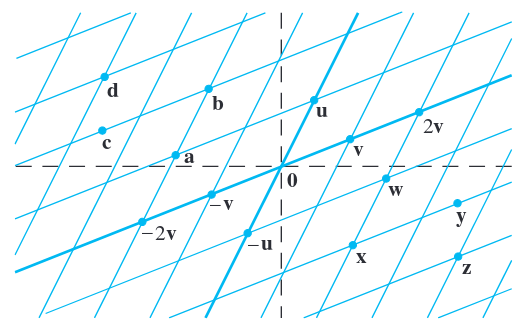
\includegraphics[width=5in]{figures/1_3_7.png}
        \end{center}
    \end{figure}

    \begin{solution}
        \begin{equation*}
            \Vect{a} = \Vect{u} - 2\Vect{v}
        \end{equation*}
        \begin{equation*}
            \Vect{b} = 2\Vect{u} - 2\Vect{v}
        \end{equation*}
        \begin{equation*}
            \Vect{c} = 2\Vect{u} - \frac{7}{2}\Vect{v}
        \end{equation*}
        \begin{equation*}
            \Vect{d} = 3\Vect{u} - 4\Vect{v}
        \end{equation*}
    \end{solution}
\end{problem}

\begin{problem}[1.3\#9]
    Write a vector equation that is equivalent to the given system of equations.
    \begin{align*}
        x_2 + 5x_3 &= 0 \\
        4x_1 + 6x_2 - x_3 &= 0 \\
        -x_1 + 3x_2 - 8x_3 &= 0
    \end{align*}

    \begin{solution}
        The vector equation that is equivalent to the given system of equations is
        \begin{equation*}
            x_1 \begin{bmatrix}
                0 \\ 4 \\ -1
            \end{bmatrix} + x_2 \begin{bmatrix}
                1 \\ 6 \\ 3
            \end{bmatrix} + x_3 \begin{bmatrix}
                5 \\ -1 \\ -8
            \end{bmatrix} = \begin{bmatrix}
                0 \\ 0 \\ 0
            \end{bmatrix}
        \end{equation*}
    \end{solution}
\end{problem}

\begin{problem}[1.3\#13]
    Determine if $\Vect{b}$ is a linear combination of the vectors formed from the columns of the matrix $A$.
    \begin{equation*}
        A = \begin{bmatrix}
            1 & -4 & 2 \\
            0 & 3 & 5 \\
            -2 & 8 & -4
        \end{bmatrix},
        \Vect{b} = \begin{bmatrix}
            3 \\ -7 \\ -3
        \end{bmatrix}
    \end{equation*}

    \begin{solution}
        \begin{align*}
            \begin{bmatrix}
                1 & -4 & 2 & 3 \\
                0 & 3 & 5 & 7 \\
                -2 & 8 & -4 & -3
            \end{bmatrix}
            & \equiv
            \begin{bmatrix}
                1 & -4 & 2 & 3 \\
                0 & 3 & 5 & 7 \\
                0 & 0 & 0 & 3
            \end{bmatrix}
            & R3 = 2 * R1 + R3
        \end{align*}

        $\Vect{b}$ is not a linear combination of the vectors formed from the columns of the matrix A.
    \end{solution}
\end{problem}

\begin{problem}[1.3\#17]
    Let $\Vect{a_1} = \begin{bmatrix}1 \\ 4 \\ -2\end{bmatrix}$, 
    $\Vect{a_2} = \begin{bmatrix}-2 \\ -3 \\ 7\end{bmatrix}$, and
    $\Vect{b} = \begin{bmatrix}4 \\ 1 \\ h\end{bmatrix}$. For what value(s) of $h$ is $\Vect{b}$ in the plane spanned by $\Vect{a_1}$ and $\Vect{a_2}$?

    \begin{solution}
        \begin{align*}
            \begin{bmatrix}
                1 & -2 & 4 \\
                4 & -3 & 1 \\
                -2 & 7 & h
            \end{bmatrix}
            & \equiv
            \begin{bmatrix}
                1 & -2 & 4 \\
                4 & -3 & 1 \\
                0 & 3 & h + 8
            \end{bmatrix}
            & R3 = 2 * R1 + R3 \\ & \equiv
            \begin{bmatrix}
                1 & -2 & 4 \\
                0 & 5 & -15 \\
                0 & 3 & h + 8
            \end{bmatrix}
            & R2 = -4 * R1 + R2 \\ & \equiv
            \begin{bmatrix}
                1 & -2 & 4 \\
                0 & 1 & -3 \\
                0 & 3 & h + 8
            \end{bmatrix}
            & R2 = \frac{1}{5} R2 \\ & \equiv
            \begin{bmatrix}
                1 & -2 & 4 \\
                0 & 1 & -3 \\
                0 & 0 & h + 17
            \end{bmatrix}
            & R3 = -3 * R2 + R3 \\ & \equiv
            \begin{bmatrix}
                1 & 0 & -2 \\
                0 & 1 & -3 \\
                0 & 0 & h + 17
            \end{bmatrix}
            & R1 = 2 * R2 + R1
        \end{align*}

        In order for $\Vect{b}$ to be in the splane spanned by $\Vect{a_1}$ and $\Vect{a_2}$, $h + 17 = 0$, so $h = -17$.
    \end{solution}
\end{problem}

\pagebreak
\begin{problem}[1.3\#19]
    Give a geometric description of the Span $\{\Vect{v_1}, \Vect{v_2}\}$ for vectors 
    $\Vect{v_1} = \begin{bmatrix}3 \\ 0 \\ 2\end{bmatrix}$,
    $\Vect{v_2} = \begin{bmatrix}-2 \\ 0 \\ 3\end{bmatrix}$

    \begin{solution}
        The geometric description of the Span $\{\Vect{v_1}, \Vect{v_2}\}$ is the plane that contains the vectors $\begin{bmatrix}3 \\ 0 \\ 2\end{bmatrix}$ and $\begin{bmatrix}-2 \\ 0 \\ 3\end{bmatrix}$ and passes through the origin.
    \end{solution}
\end{problem}

\begin{problem}[1.3\#24]
    Determine whether each statement is True or False. Justify your answer.
    \begin{enumerate}[label=(\alph*)]
        \item Any list of five real numbers is a vector in $\R^5$.
        \item The vector $\Vect{u}$ results when a vector $\Vect{u} - \Vect{v}$ is added to the vector $\Vect{v}$.
        \item The weights $c_1,\ldots,c_p$ in a linear combination $c_1\Vect{v_1}, \ldots, c_p\Vect{v_p}$ cannot be all zero.
        \item When $\Vect{u}$ and $\Vect{v}$ are nonzero vectors, Span $\{\Vect{u}, \Vect{v}\}$ contains the line through $\Vect{u}$ and the origin.
        \item Asking whether the linear system corresponding to an augmented matrix $\begin{bmatrix}\Vect{a_1} & \Vect{a_2} & \Vect{a_3} & \Vect{b}\end{bmatrix}$ has a solution amounts to asking if $\Vect{b}$ is in Span $\{\Vect{a_1}, \Vect{a_2}, \Vect{a_3}\}$
    \end{enumerate}

    \begin{solution}
        \begin{enumerate}[label=(\alph*)]
            \item \underline{True}, $\R^n$ is the set of all lists or real numbers of length $n$.
            \item \underline{True}, $(\Vect{u} - \Vect{v}) + \Vect{v} = \Vect{u} + (\Vect{v} - \Vect{v}) = \Vect{u}$. 
            \item \underline{False}, the zero matrix is a linear combination of any set of vectors with zero weights.
            \item \underline{True}, the Span $\{\Vect{u}, \Vect{v}\}$ contains all points that are a linear combination of $\Vect{u}$ and $\Vect{v}$ and all the points on the line through $\Vect{u}$ and the origin are a linear combination of $\Vect{u}$ and $\Vect{v}$.
            \item \underline{True}, if $\Vect{b}$ is in Span $\{\Vect{a_1}, \Vect{a_2}, \Vect{a_3}\}$, then there is some linear combination of $\Vect{a_1}, \Vect{a_2}, \Vect{a_3}$ that is equal to $\Vect{b}$, and in order for a linear combination to exist there must be a solution to the linear system.
        \end{enumerate}
    \end{solution}
\end{problem}

\pagebreak
\begin{problem}[1.3\#25]
    Let $A = \begin{bmatrix}
        1 & 0 & -4 \\
        0 & 3 & -2 \\
        -2 & 6 & 3
    \end{bmatrix}$ and $\Vect{b} = \begin{bmatrix}4 \\ 1 \\ -4\end{bmatrix}$. Denote the columns of $A$ by $\Vect{a_1}$, $\Vect{a_2}$, $\Vect{a_3}$, and let $W = $ Span $\{\Vect{a_1},\Vect{a_2},\Vect{a_3}\}$.
    
    \begin{enumerate}[label=(\alph*)]
        \item is $\Vect{b}$ in $\{\Vect{a_1},\Vect{a_2},\Vect{a_3}\}$? How many vectors are in $\{\Vect{a_1},\Vect{a_2},\Vect{a_3}\}$?
        \item is $\Vect{b}$ in $W$? How many vectors are in $W$?
        \item Show that $\Vect{a_1}$ is in $W$. [Hint: Row operations are unnecessary.]
    \end{enumerate}

    \begin{solution}
        \begin{enumerate}[label=(\alph*)]
            \item No, there are three vectors in the set $\{\Vect{a_1}, \Vect{a_2}, \Vect{a_3}\}$
            \item Yes, there are an infinite number of vectors in $W$.
            \item The vector $\Vect{a_1}$ can be written as a linear combination of $\Vect{a_1}$, $\Vect{a_2}$, $\Vect{a_3}$, so it is in $W$ ($\Vect{a_1} = 1\Vect{a_1} + 0 \Vect{a_2} + 0 \Vect{a_3}$).
        \end{enumerate}
    \end{solution}
\end{problem}

\pagebreak
\begin{problem}[1.3\#29]
    Let $v_1,\ldots,v_k$ be points in $\R^3$ and supposed that for $j = 1,\ldots,k$ an object with mass $m_j$ is located at point $v_j$.
    Physicists call such objects \textit{point masses}. The total mass of the system of point masses is
    \begin{equation*}
        m = m_1 + \ldots + m_k
    \end{equation*}
    The \textit{center of mass} of the system is
    \begin{equation*}
        \Vect{v} = \frac{1}{m}(m_1v_1 + m_2v_2 + \ldots + m_kv_k)
    \end{equation*}
    Compute the center of gtavity of the system consisting of the following point masses
    \begin{figure}[H]
        \begin{center}
            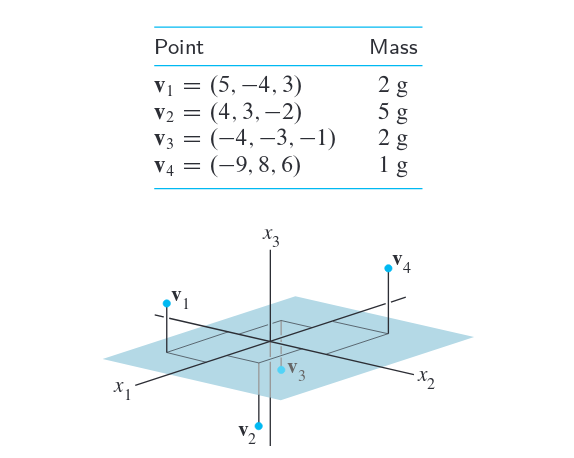
\includegraphics[width=5in]{figures/1_3_29.png}
        \end{center}
    \end{figure}

    \begin{solution}
        \begin{equation*}
            \Vect{v} = \frac{1}{10}(2\begin{bmatrix}
                5 \\ -4 \\ 3
            \end{bmatrix} + 5 \begin{bmatrix}
                4 \\ 3 \\ -1
            \end{bmatrix} + 2 \begin{bmatrix}
                -4 \\ -3 \\ -1
            \end{bmatrix} + \begin{bmatrix}
                -9 \\ 8 \\ 6
            \end{bmatrix}) = \begin{bmatrix}
                \frac{13}{10} \\ \frac{9}{10} \\ 0
            \end{bmatrix}
        \end{equation*}

        The center of mass of the system is at $(\frac{13}{10}, \frac{9}{10}, 0)$.
    \end{solution}
\end{problem}

\pagebreak
\begin{problem}[1.3\#34]
    Use the vector $\Vect{u} = (u_1, \ldots, u_n)$ to verify the following algebraic properties of $\R^n$.
    \begin{enumerate}[label=(\alph*)]
        \item $\Vect{u} + (-\Vect{u}) = (-\Vect{u}) + \Vect{u} = 0$
        \item $c(d\Vect{u}) = (cd)\Vect{u}$ for all scalars c and d
    \end{enumerate}

    \begin{solution}
        \begin{proof}
            $\Vect{u} + (-\Vect{u}) = (-\Vect{u}) + \Vect{u}$

            \begin{align*}
                \Vect{u} + (-\Vect{u}) & = (u_1, \ldots, u_n) - (u_1, \ldots, u_n) & \By{substution} \\
                & = (u_1 - u_1, \ldots, u_n - u_n) & \By{vector addition} \\
                & = ((-u_1) + u_1, \ldots, (-u_n) + u_n) & \By{associative property of addition} \\
                & = (-\Vect{u}) + \Vect{u} & \By{vector addition}
            \end{align*}
        \end{proof}

        \begin{proof}
            $\Vect{u} + (-\Vect{u}) = 0$

            \begin{align*}
                \Vect{u} + (-\Vect{u}) & = (u_1, \ldots, u_n) - (u_1, \ldots, u_n) & \By{substution} \\
                & = (u_1 - u_1, \ldots, u_n - u_n) & \By{vector addition} \\
                & = (0, \ldots, 0) & \By{addition} \\
                & = 0 & \By{def. of zero vector}
            \end{align*}
        \end{proof}

        \begin{proof}
            $c(d\Vect{u}) = (cd)\Vect{u}$ for all scalars c and d

            \begin{align*}
                c(d\Vect{u}) & = c(du_1, \ldots, cu_n) & \By{scalar multiplication} \\
                & = (c(du_1), \ldots, c(cu_n)) & \By{scalar multiplication of vector} \\
                & = ((cd)u_1, \ldots, (cd)u_n) & \By{communative property of multiplication} \\
                & = (cd)\Vect{u} & \By{scalar multiplication of vector}
            \end{align*}
        \end{proof}
    \end{solution}
\end{problem}

\end{document}
